\section{ETVOIP}
No separador ETVOIP de uma máquina virtual é possibilitada a gestão VOIP de uma solução ETVOIP.
Actualmente o ETVOIP consiste na interação com o componente PBX podendo de futuro interagir com outros desenvolvidos.
Os módulos disponíveis por este agente são:
\begin{itemize}
    \item Extensões
    \item Trunks
    \item Rotas de Saída
    \item Rotas de Entrada
\end{itemize}


\begin{quote}
	{\large \bf Nota} \\*[-.8pc]
	\underline{\hspace{6in}} \\
    No fim de todas as operações/alterações efectuadas deverá usar a opção \emph{Aplicar Alterações} disponível em qualquer um dos módulos de forma a reflectir essas alterações na configuração actual do sistema VOIP.
\end{quote}


\begin{figure}[H]
        \begin{center}
        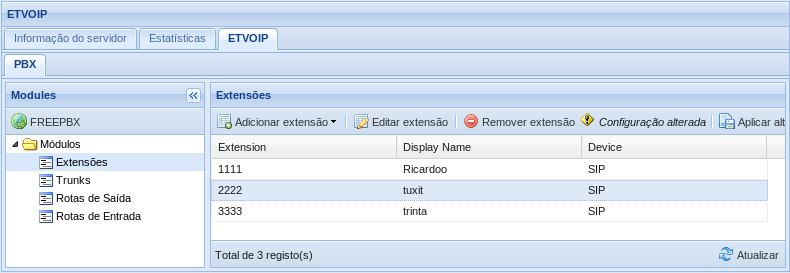
\includegraphics[scale=0.4]{screenshots/etvoip_pbx.png}
        \caption{Painel principal de gestão ETVOIP}
        \label{fig:etvoip_pbx}
        \end{center}
\end{figure}

Para além destes módulos existe também a opção de abrir isoladamente o FREEPBX numa janela, podendo aceder a configurações avançadas (Menu FREEPBX).


\subsection{Extensões}

Em \emph{Extensões} é possível efectuar operações de adicionar/editar e remover extensões.

\begin{quote}
	{\large \bf Nota} \\*[-.8pc]
	\underline{\hspace{6in}} \\
    Apenas é possível criar/editar extensões do tipo SIP\footnote{SIP é um protocolo standar usado para dispositivos VoIP} e/ou IAX\footnote{IAX é um protocolo "Inter Asterisk" usado para interligação servidores asterisk.}.
\end{quote}

\begin{figure}[H]
        \begin{center}
        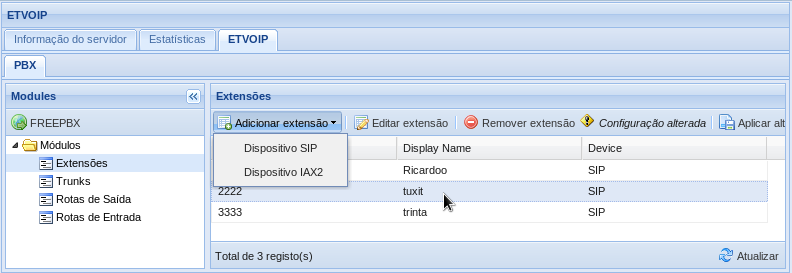
\includegraphics[scale=0.4]{screenshots/etvoip_pbx_extensions.png}
        \caption{Painel de gestão de Extensões}
        \label{fig:etvoip_pbx_extensions}
        \end{center}
\end{figure}


\subsubsection{Adicionar Extensão}
\label{sec:etvoip_pbx_extensions_add}

Ao criar uma extensão é possível optar entre a vista de configuração básica/avançada dos parâmetros da extensão.

\begin{figure}[H]
        \begin{center}
        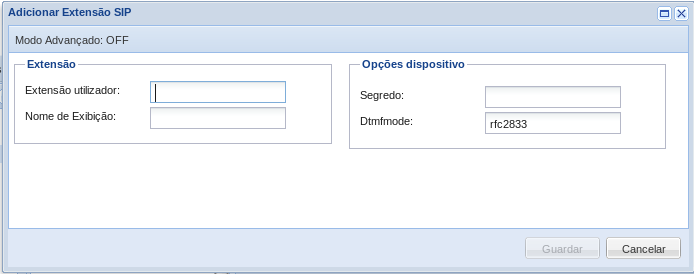
\includegraphics[scale=0.4]{screenshots/etvoip_pbx_extensions_sip.png}
        \caption{Janel de criação de extensão SIP}
        \label{fig:etvoip_pbx_extensions_sip}
        \end{center}
\end{figure}


\begin{description}
	\item[Modo Avançado: OFF -] Neste modo é disponibilizado apenas os campos básicos de criação de uma extensão.
        \begin{description}
            \item[Extensão -] Parâmetros de definição da extensão.
                \begin{itemize}
                    \item Extensão utilizador - Número de extensão a marcar para alcançar este utilizador. Deve ser única.
                    \item Nome de Exibição - A identificação usada nas chamadas efectuadas por este utilizador. Introduzir um nome, não um número.
                \end{itemize}

            \item[Opções dispositivo -] Opções relativas ao tipo de dispositivo escolhido.
                \begin{itemize}
                    \item Segredo - Password utilizada pelos dispositivos telefónicos para autenticar no servidor asterisk.
                    \item Dtmfmode - Frequência Multi Dual-Tone
                        \begin{itemize}
                            \item inband - O dispositivo telefónico de envio gera os tons DTMF.
                            \item outband - Os tons de toque são removidos dos dados aúdio e enviados por um canal diferente.
                            \item rfc2833 - Especifica um formato de envio de pacotes RTP, de forma a reduzir os dados transmitidos. Usada por defeito.
                        \end{itemize}
                \end{itemize}
        \end{description}
	\item[Modo Avançado: ON -] Neste modo para além dos parâmetros já mencionados é possível configurar os seguintes:
        \begin{description}
            \item[Extensão -] Parâmetros de definição da extensão.
                \begin{itemize}
                    \item Número CID Alternativo - Número CID a ser utilizado em chamadas internas, se diferente do número de extensão. Utilizado para mascarar como um utilizador diferente. Um exemplo comum é quando uma equipa tèncica necessita de ter o seu caller ID interno a mostrar o número geral de suporte. Não tem efeito nas chamadas externas.
                    \item SIP Alternativo - Se quiser ter suporte a chamadas sip directas a utilizadores internos ou através de chamadas sip anónimas, pode fornecer um nome amigável que pode ser usado em vez da extensão do utilizador.
                \end{itemize}

            \item[Opções de extensão -] Opções avançadas de uma extensão.
                \begin{itemize}
                    \item Outbound CID - Substitui a identificação de chamada se passar um trunk. Sobrepôe ao outbound CID do trunk.
                    \item Tempo de chamada - Número de segundos a tocar antes de enviar a chamada para o voicemail. Se não tiver configurado voicemail este parametro será ignorado.
                    \item Chamada em Espera - Configura o estado inicial de "chamada em espera" para esta extensão (\emph{Disable} ou \emph{Enable})
                    \item Triagem de chamada - Exige que um utilizador externo diga o seu nome, que será depois ouvido pelo utilizador, permitindo aceitar ou rejeitar a chamada. Triagem com memória (\emph{Screen Caller: Memory}) verifica apenas uma vez a origem do identificador de chamada. Triagem sem memória (\emph{Screen Caller: No Memory}) requer sempre que o utilizador externo diga o seu nome. Qualquer dos modos anunciará sempre o utilizador a partir da última introdução guardada com essa identificação de chamada.
                    \item Marcação sem PIN - Habilitado permite efectuar chamadas de saída a partir desta extensão sem marcação de PIN
                    \item CID de Emergência - Este identificador de chamada será usado sempre que se marque uma rota de saída marcada como saída como Emergência. O CID de Emergência substitui todas as outras configurações da identificação de chamada.
                \end{itemize}

            \item[Atribuição DID/CID -] Definição de rota de entrada para esta extensão.
                \begin{itemize}
                    \item Descrição DID - Descrição da rota de entrada.
                    \item Adicionar DID entrada - Define o número (Direct Inward Dialing) de entrada associado a esta extensão.
                    \item Adicionar CID entrada - Permite especificar melhor uma rota DID + CID. DID deve ser especificado no parâmetro acima.
                \end{itemize}

            \item[Voicemail \& Directoria -] Parâmetros de configuração do voicemail.
                \begin{itemize}
                    \item Estado - Habilita/desabilita o voicemail nesta extensão.
                    \item Voicemail Password - Password de acesso ao sistema de voicemail. A password só pode conter números. Um utilizador pode alterar a password introduzida aqui após aceder ao sistema de voicemail (*98) via telefone.
                    \item Endereço Email - Endereço de email de destino para onde são enviadas notificações de voicemails.
                    \item Endereço Email Pager - Endereço email pager/telemóvel para envio de pequenas notificações de voicemail.
                    \item Anexar Email - Permite anexar os voicemails ao email.
                    \item Tocar CID - Lê o número de telefone de origem antes de tocar a mensagem de entrada.
                    \item Tocar Envelope - Controla se é lida a data/hora da mensagem.
                    \item Apagar Voicemail - Se activado a mensagem será apagada do voicemailbox (após ter sida enviada por email). Permite a um utilizador recer voicemail via email, sem ter que recuperar o voicemail via interface web ou telefone.  PRECAUÇÂO: NECESSITA TER voicemail anexado ao email CASO CONTRÁRIO AS MENSAGENS SERÂO PERDIDAS.
                    \item Utilizador IMAP - Utilizador IMAP caso use IMAP
                    \item Password IMAP - Password IMAP
                    \item Opções VM - Opções extra do voicemail separadas por | (tais como review=yes|maxmessage=60).
                    \item Contexto VM - Contexto usado pelo sistema de voicemail. Use 'default' caso não saiba as suas implicações.
                \end{itemize}

            \item[Serviços dicção -] Parâmetros do serviço de dicção. Se habilitado, permite ao utilizador marcar *34 do seu telefone e gravar o que for dito. A mensagem será gravada no formato definido e enviada para o email especificado.
                \begin{itemize}
                    \item Serviço Dicção
                    \item Formato Dicção
                    \item Endereço Email
                \end{itemize}

            \item[Idioma -] Parâmetros de idioma da extensão.
                \begin{itemize}
                    \item Código de idioma - Irá perguntar se pretende usar o idioma seleccionado, se instalado
                \end{itemize}

            \item[Opções de gravação -] Parâmetros de gravação da extensão.
                \begin{itemize}
                    \item Registo de entrada - Regista todas as chamadas de entrada desta extensão.
                    \item Registo de saída - Regista todas as chamadas de saída desta extensão.
                \end{itemize}
            
        \end{description}
\end{description}

\subsubsection{Editar extensão}

Para editar uma extensão é necessário seleccionar a extensão pretendida e clica-se em \emph{Editar extensão}. Surgirá então uma janela (ver figura \ref{fig:etvoip_pbx_extensions_sip}) preenchida com as definições da extensão.
Os parâmetros disponibilizados são idênticos aos da secção \ref{sec:etvoip_pbx_extensions_add}.

\subsubsection{Remover extensão}

Para remover uma extensão selecciona-se a extensão a eliminar e clica-se em \emph{Remover extensão}.
Surgirá uma janela de confirmação de remoção da extensão (figura \ref{fig:etvoip_pbx_extensions_remove}). Após a remoção da extensão e caso não se pretenda efectuar nenhuma outra operação, deverá aplicar as alterações efectuadas - \emph{Aplicar alterações}.

\begin{figure}[H]
        \begin{center}
        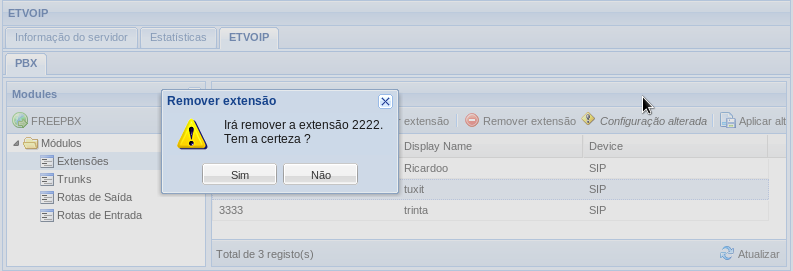
\includegraphics[scale=0.4]{screenshots/etvoip_pbx_extensions_remove.png}
        \caption{Remover extensão}
        \label{fig:etvoip_pbx_extensions_remove}
        \end{center}
\end{figure}

\subsection{Trunks}

Em \emph{Trunks} é possível efectuar operações de adicionar/editar e remover trunks.

\begin{quote}
	{\large \bf Nota} \\*[-.8pc]
	\underline{\hspace{6in}} \\
    Apenas é possível criar/editar trunks do tipo SIP e/ou IAX.
\end{quote}

\begin{figure}[H]
        \begin{center}
        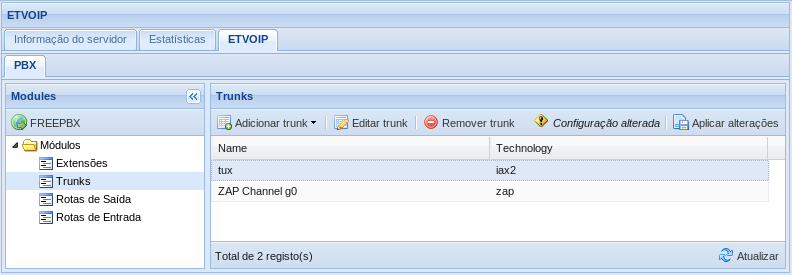
\includegraphics[scale=0.4]{screenshots/etvoip_pbx_trunks.png}
        \caption{Painel de gestão de Trunks}
        \label{fig:etvoip_pbx_trunks}
        \end{center}
\end{figure}

\subsubsection{Adicionar Trunk}
\label{sec:etvoip_pbx_trunks_add}

Ao criar um trunk é possível optar entre a vista de configuração básica/avançada dos parâmetros da trunk.

\begin{figure}[H]
        \begin{center}
        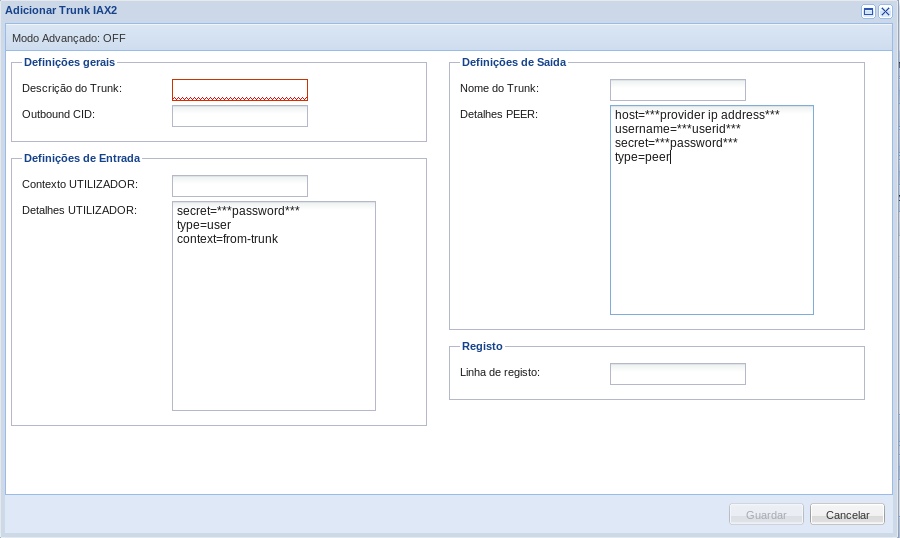
\includegraphics[scale=0.4]{screenshots/etvoip_pbx_trunks_iax.png}
        \caption{Janel de criação de trunk IAX2}
        \label{fig:etvoip_pbx_trunks_iax}
        \end{center}
\end{figure}


\begin{description}
	\item[Modo Avançado: OFF -] Neste modo é disponibilizado apenas os campos básicos de criação de um trunk.
        \begin{description}
            \item[Definições gerais -] Parâmetros de definição do trunk.
                \begin{itemize}
                    \item Descrição do Trunk - Nome descritivo para a trunk.
                    \item Outbound CID - Identificador de chamada usado em chamadas efectuadas por este trunk.
                \end{itemize}

            \item[Definições de Entrada -] Opções relativas à configuração de entrada do trunk.
                \begin{itemize}
                    \item Contexto UTILIZADOR - Isto é geralmente o nome da conta ou número que o provedor está à espera. Este Contexto UTILIZADOR é usado para definir os detalhes do utilizador abaixo definidos.
                    \item Detalhes UTILIZADOR - Parâmetros de ligação do UTILIZADOR ao sistema VOIP.                        
                \end{itemize}
            \item[Definições de Saída -] Opções relativas à configuração de saída do trunk.
                \begin{itemize}
                    \item Nome do trunk - Nome único do trunk.
                    \item Detalhes PEER - Parâmetros de ligação do PEER ao sistema VOIP.
                \end{itemize}
            \item[Registo -] Definição de registo num VoIP.
                \begin{itemize}
                    \item Linha de registo - Muitos provedores VoIP requerem que o sistema se REGISTE. Introduza a linha de registo aqui (exemplo: username:password@switch.voipprovider.com).Muitos provedores requerem um número DID, (ex: username:password@switch.voipprovider.com/didnumber) para que funcione a correspondência DID
                \end{itemize}
        \end{description}
	\item[Modo Avançado: ON -] Neste modo para além dos parâmetros já mencionados é possível configurar os seguintes:
        \begin{description}
            \item[Definições gerais -] Parâmetros de definição do trunk.
                \begin{itemize}
                    \item Opções CID - Determina os CIDs que serão permitidos neste trunk. IMPORTANTE: CIDs de emergência definidos numa extensão serão sempre usados se o trunk fizer parte de uma rota de EMERGENCIA independentemente das configurações:
                        \begin{itemize}
                            \item Allow Any CID - Todos os CIDs incluindo os provenientes de chamadas externas reencaminhadas serão transmitidos.
                            \item Block Foreign CIDs - Bloqueia CIDs que sejam provenientes de chamadas reencaminhadas para o sistema. CIDs defindos para estensões serão transmitidos.
                            \item Remove CNAM - Esta opção removerá CNAM de cada CID enviado por este trunk.
                            \item Force Trunk CID - Utiliza sempre o CID definido para este trunk excepto se fizer parete de uma rota de emergência com um CID de emergência definido para uma extensão.
                        \end{itemize}                         
                    \item Limite de canais - Controla o número máximo de canais de saída (chamadas simultâneas) que podem ser usados por este trunk. Chamadas de entrada não são consideradas. Deixe em branco para não especificar um limite.
                    \item Desabilitar Trunk - Desabilita o uso deste trunk em todas rotas em que é usado.
                    \item Monitorizar Falhas no Trunk - Se habilitado, introduza o nome de um script AGI que será usado para log, email ou efectuar uma acção qualquer caso as falhas não são causadas por NOANSWER ou CANCEL.
                \end{itemize}

            \item[Regras de marcação de saída -] Opções avançadas de marcação num trunk.
                \begin{itemize}
                    \item Regras de marcação - Uma regra de marcação controla o modo como as chamadas serão marcadas neste trunk. Pode ser usada para adicionar ou remover prefixos. Os números que não fizerem correspondência com os padrões definidos aqui serão marcados sem alteração. Um padrão sem + ou | (para adicionar ou remover um prefixo) não fará alterações mas irá criar uma correspondência. Apenas a primeira correspondência encontrada será executada sem executar as restantes regras:
                        \begin{itemize}
                            \item X - Faz correspondência com digitos entre 0-9.
                            \item Z - Faz correspondência com digitos entre 1-9.
                            \item N - Faz correspondência com digitos entre 2-9.
                            \item [1237-9] - Faz correspondência com digitos ou letras entre parêntesis (neste exemplo, 1,2,3,7,8,9).
                            \item . - Wildcard, faz correspondência com um ou mais caracteres (não permitido antes de | ou +).
                            \item | - Remove um prefixo de marcação do número (por exemplo, 613|NXXXXXX tem correspondência quando alguém marca "6135551234" mas apenas passa "5551234" para o trunk).
                            \item + - Adiciona um prefixo de marcação ao número (por exemplo, 1613+NXXXXXX tem correspondência quando alguém marca "5551234" e passa "16135551234" para o trunk).
                        \end{itemize}
                        Pode-se usar simultâneamente + e |, por examplo: 01+0|1ZXXXXXXXXX faz correspondência com "016065551234" e marca como "0116065551234" Note que a ordem não interessa, ou seja, 0|01+1ZXXXXXXXXX faz exactamente a mesma coisa.

                    \item Prefixo de marcação Outbound - O prefixo de outbound é usado para colocar um prefixo em todas as chamadas de saída deste trunk. Por exemplo, se este trunk tiver por detràs de outro PBX, podemos usar o 9 para aceder a uma linha de saída. A maior parte dos utilizadores deverão deixar a opção em branco.
                \end{itemize}
        \end{description}
\end{description}


\subsubsection{Editar trunk}

Para editar um trunk é necessário seleccionar a trunk pretendida e clica-se em \emph{Editar trunk}. Surgirá então uma janela (ver figura \ref{fig:etvoip_pbx_trunks_iax}) preenchida com as definições do trunk.
Os parâmetros disponibilizados são idênticos aos da secção \ref{sec:etvoip_pbx_trunks_add}.

\subsubsection{Remover trunk}

Para remover um trunk selecciona-se o trunk a eliminar e clica-se em \emph{Remover trunk}.
Surgirá uma janela de confirmação de remoção do trunk (figura \ref{fig:etvoip_pbx_trunks_remove}). Após a remoção do trunk e caso não se pretenda efectuar nenhuma outra operação, deverá aplicar as alterações efectuadas - \emph{Aplicar alterações}.

\begin{figure}[H]
        \begin{center}
        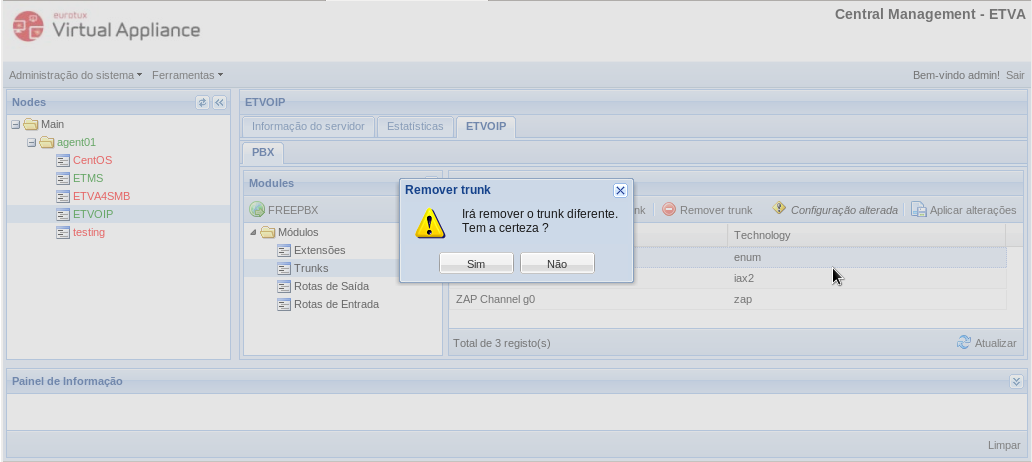
\includegraphics[scale=0.4]{screenshots/etvoip_pbx_trunks_remove.png}
        \caption{Remover trunk}
        \label{fig:etvoip_pbx_trunks_remove}
        \end{center}
\end{figure}


\subsection{Rotas de Saída}

Em \emph{Rotas de Saída} configura-se o comportamento das chamadas de saída (chamadas para o exterior). O número marcado é analizado, e ao fazer correspondência
com determinado padrão de marcação de uma rota, é encaminhado para a respectiva trunk.

É possível efectuar operações de adicionar, editar e remover rotas de saída.

\begin{figure}[H]
        \begin{center}
        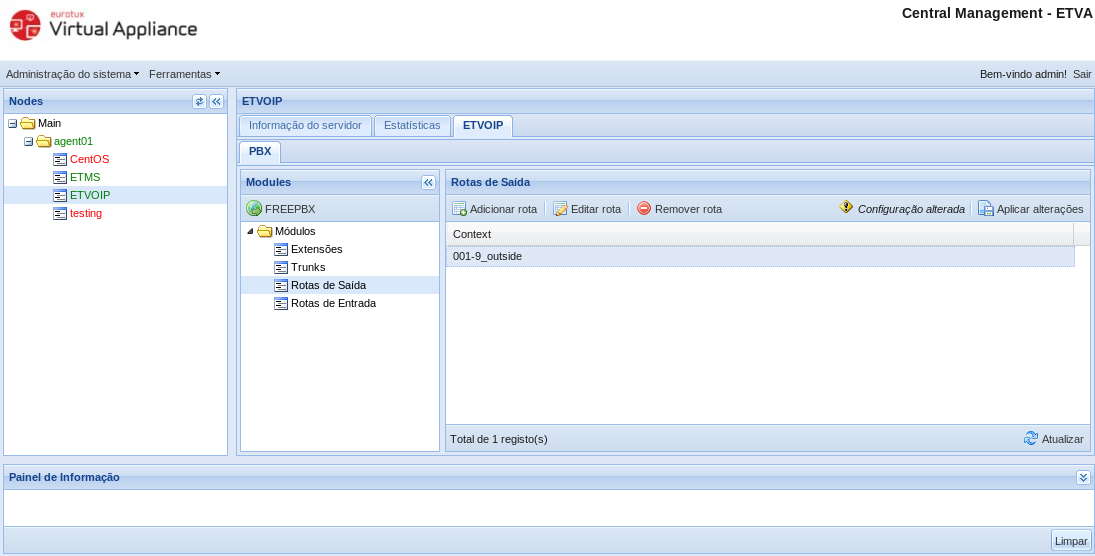
\includegraphics[scale=0.4]{screenshots/etvoip_pbx_outbound_routes.png}
        \caption{Painel de gestão de Rotas de Saída}
        \label{fig:etvoip_pbx_outbound_routes}
        \end{center}
\end{figure}

\subsubsection{Adicionar Rota}
\label{sec:etvoip_pbx_outbound_routes_add}

Ao seleccionar \emph{Adicionar rota} surgirá uma janela (ver figura \ref{fig:etvoip_pbx_outbound_routes_add}) onde é possível optar entre a vista de configuração básica/avançada dos seguintes parâmetros:

\begin{description}
	\item[Modo Avançado: OFF -] Neste modo é disponibilizado apenas os campos básicos de criação de uma rota.
        \begin{description}
            \item[Definições gerais -] Parâmetros de definição da rota.
                \begin{itemize}
                    \item Nome da rota - Nome descritivo para a rota (por exemplo, 'local' ou 'longa-distancia').
                    \item Padrões de Marcação - Um padrão de marcação é uma combinação única de digitos que seleccionarão este trunk:
                        \begin{itemize}
                            \item X - Faz correspondência com digitos entre 0-9.
                            \item Z - Faz correspondência com digitos entre 1-9.
                            \item N - Faz correspondência com digitos entre 2-9.
                            \item [1237-9] - Faz correspondência com digitos ou letras entre parêntesis (neste exemplo, 1,2,3,7,8,9).
                            \item . - Wildcard, faz correspondência com um ou mais caracteres.
                            \item | - Separa o prefixo de marcação do número (por exemplo, 9|NXXXXXX faz correspondência com "95551234" mas apenas passa "5551234" para os trunks).
                            \item / - Adiciona ao padrão de marcação, faz correspondência com um CID ou um padrão (por exemplo, NXXXXXX/104 faz correspondência apenas com a extensão "104").
                        \end{itemize}                                            
                \end{itemize}

            \item[Trunks -] Sequência de trunks de saída. A sequência de trunks controla a ordem das trunks que serão usadas quando houver correspondência com os padrões de marcação acima definidos.
                            Para padrões de marcação que fazem correspondência com números usados em chamadas internacionais, por exemplo, será pretendido que se use a rota mais barata para chamadas de longa distância (ie, primeiro trunks VoIP) seguido pelas rotas mais caras (linhas POTS).
        \end{description}
	\item[Modo Avançado: ON -] Neste modo para além dos parâmetros já mencionados é possível configurar os seguintes:
        \begin{description}
            \item[Definições gerais -] Parâmetros de definição do trunk.
                \begin{itemize}
                    \item CID da rota - Se definida, irá reescrever todos os CIDs especificados excepto:
                        \begin{itemize}
                            \item CIDs de emergência de extensão/dispositivo se esta rota tiver marcada como rota de emergência.
                            \item CID do trunk se o trunk está marcado para forçar CID.
                            \item CIDs de chamadas reencaminhadas (CF, Follow Me, Ring Groups, etc).
                            \item CIDs de extensões/utilizadores se habilitados.
                        \end{itemize}                       
                    \item Password da rota - A rota pode requisitar ao utilizador uma password antes de autorizar a chamada. Torna-se útil nos casos de restrição de chamadas internacionais.
                                             Uma password numérica, ou o caminho para um ficheiro com a password podem ser usados. Deixe este campo em branco para não ser requisitada uma password.
                    \item Marcação de Emergência - Seleccionando esta opção irá forçar o uso de um CID de emergência de um dispositivo (caso esteja configurado). Esta opção permite que um determinado conjunto de rotas seja usado para marcação do número de Emergência (p.ex: 112).
                    \item Rota Intra-Companhia - Seleccionando esta opção a rota será tratada como uma ligação intra-companhia, preservando a informação do CID interno e não usando o CID de saída quer da extensão ou trunk.
                    \item Música em Espera - Define a categoria da música a tocar quando a chamada se encontra em espera.
                \end{itemize}            
        \end{description}
\end{description}


\begin{figure}[H]
        \begin{center}
        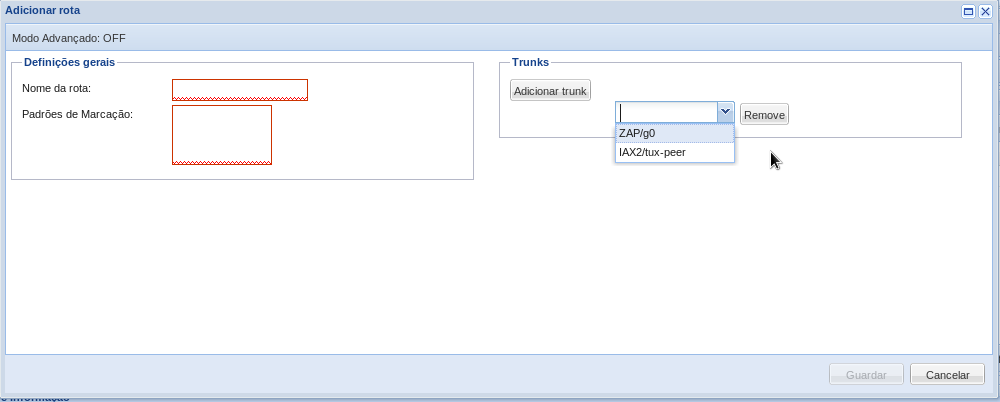
\includegraphics[scale=0.4]{screenshots/etvoip_pbx_outbound_routes_add.png}
        \caption{Janela de criação de uma rota de saída}
        \label{fig:etvoip_pbx_outbound_routes_add}
        \end{center}
\end{figure}


\subsubsection{Editar rota}

Para editar uma rota de saída é necessário seleccionar a rota pretendida e clica-se em \emph{Editar rota}. Surgirá então uma janela (ver figura \ref{fig:etvoip_pbx_outbound_routes_add}) preenchida com as definições da rota.
Os parâmetros disponibilizados são idênticos aos da secção \ref{sec:etvoip_pbx_outbound_routes_add}.

\subsubsection{Remover rota}

Para remover uma rota de saída selecciona-se a rota a eliminar e clica-se em \emph{Remover rota}.
Surgirá uma janela de confirmação de remoção da rota (figura \ref{fig:etvoip_pbx_outbound_routes_remove}). Após a remoção da rota e caso não se pretenda efectuar nenhuma outra operação, deverá aplicar as alterações efectuadas - \emph{Aplicar alterações}.

\begin{figure}[H]
        \begin{center}
        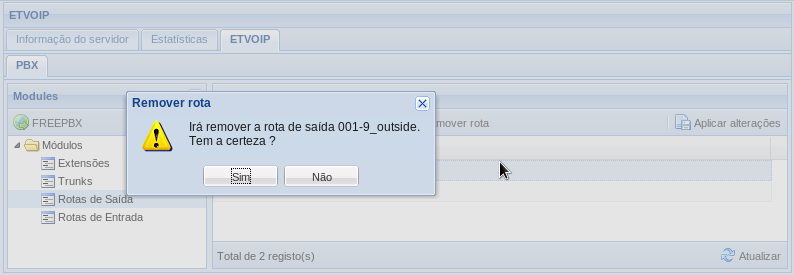
\includegraphics[scale=0.4]{screenshots/etvoip_pbx_outbound_routes_remove.png}
        \caption{Remover rota de saída}
        \label{fig:etvoip_pbx_outbound_routes_remove}
        \end{center}
\end{figure}


\subsection{Rotas de Entrada}

Em \emph{Rotas de Entrada} configura-se o comportamento das chamadas de entrada (chamdas do exterior) de todas as trunks.
Quando é recebida uma chamada de entrada, o servidor VOIP necessita saber para onde deverá direccioná-la.
Pode ser direccionada para um Ring Group, extensão ou um IVR, entre outras opções.

Sendo assim, é possível efectuar operações de adicionar, editar e remover rotas de entrada.
No painel de gestão é possível visualizar a descrição e os números DID/CID associados a cada rota.


\begin{figure}[H]
        \begin{center}
        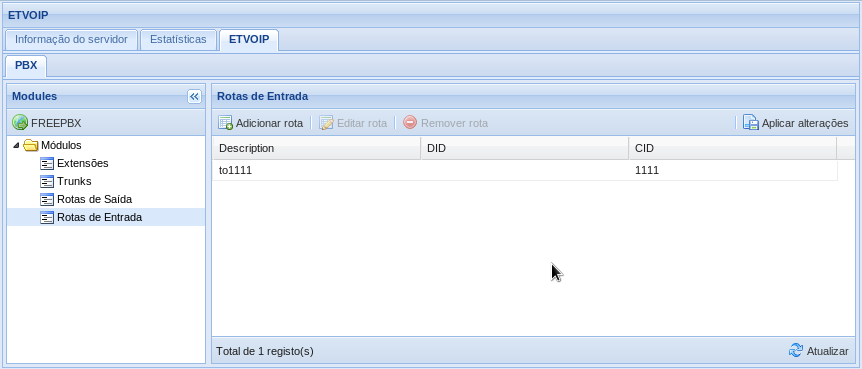
\includegraphics[scale=0.4]{screenshots/etvoip_pbx_inbound_routes.png}
        \caption{Painel de gestão de Rotas de Entrada}
        \label{fig:etvoip_pbx_inbound_routes}
        \end{center}
\end{figure}

\subsubsection{Adicionar rota}
\label{sec:etvoip_pbx_inbound_routes_add}

Ao seleccionar \emph{Adicionar rota} surgirá uma janela (ver figura \ref{fig:etvoip_pbx_inbound_routes_add} ) onde é possível configurar os seguintes parâmetros:

\begin{description}
	
            \item[Definições gerais -] Parâmetros de definição da rota.
                \begin{itemize}
                    \item \textbf{Descrição} - Nome descritivo para a rota.
                    \item \textbf{Número DID} - Define o número DID esperado se o trunk aceita DID nas chamadas de entrada. Deixe em branco para fazer correspondência com todos os DID.
                    \item \textbf{Número CID} - Define o CID para fazer correspondência nas chamadas de entrada. Deixe em branco para fazer correspondência com todos os CID.
                \end{itemize}

            \item[Definir Destino -] Destino das chamadas que fazem correspondência com o número DID/CID.
                \begin{itemize}
                    \item \textbf{Ring Groups} - Grupo de extensões.
                    \item \textbf{Terminate Call} - A chamada é automáticamente terminada.
                    \item \textbf{Phonebook Directory} - É disponibilizada a lista de contactos.
                    \item \textbf{IVR}\footnote{Acrónimo para \emph{Interactive Voice Response} (resposta interactiva de voz)} - Recepcionista virtual.
                    \item \textbf{Extensions} - Extensão pré-definida.
                \end{itemize}
       
\end{description}

\begin{figure}[H]
        \begin{center}
        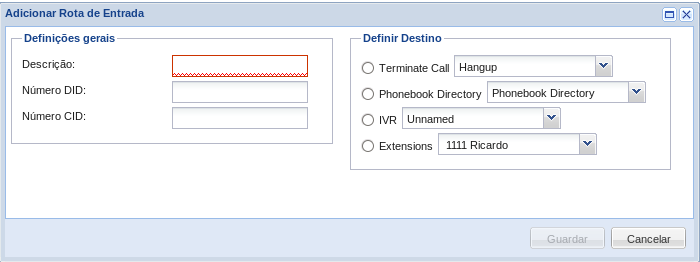
\includegraphics[scale=0.4]{screenshots/etvoip_pbx_inbound_routes_add.png}
        \caption{Janela de criação de uma rota de entrada}
        \label{fig:etvoip_pbx_inbound_routes_add}
        \end{center}
\end{figure}

\subsubsection{Editar rota}

Para editar uma rota é necessário seleccionar a rota pretendida e clica-se em \emph{Editar rota}. Surgirá então uma janela (ver figura \ref{fig:etvoip_pbx_inbound_routes_add}) preenchida com as definições da rota.
Os parâmetros disponibilizados são idênticos aos da secção \ref{sec:etvoip_pbx_inbound_routes_add}.

\subsubsection{Remover rota}

Para remover uma rota de entrada selecciona-se a rota a eliminar e clica-se em \emph{Remover rota}.
Surgirá uma janela de confirmação de remoção da rota (figura \ref{fig:etvoip_pbx_inbound_routes_remove}). Após a remoção da rota e caso não se pretenda efectuar nenhuma outra operação, deverá aplicar as alterações efectuadas - \emph{Aplicar alterações}.

\begin{figure}[H]
        \begin{center}
        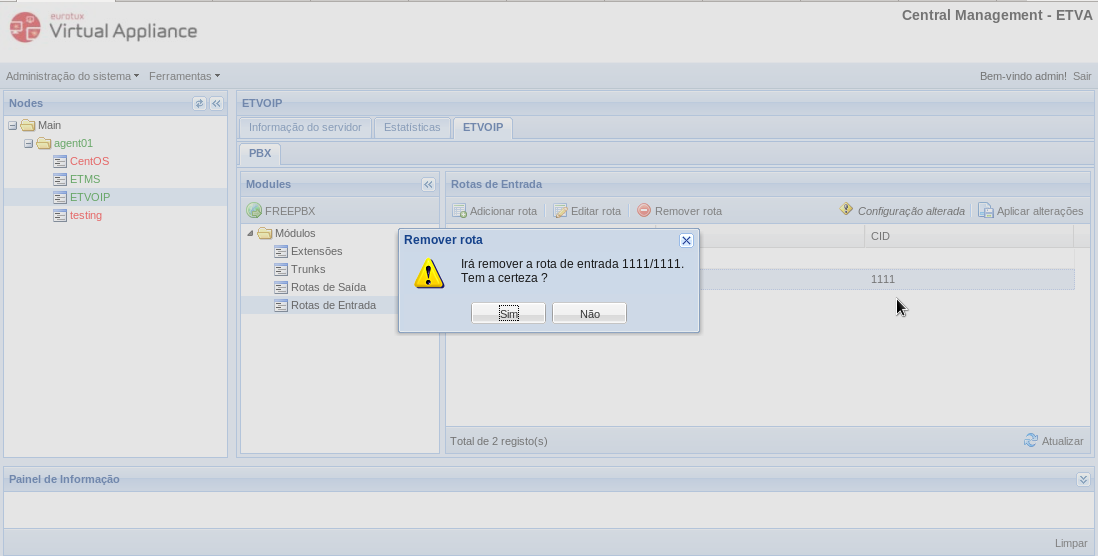
\includegraphics[scale=0.4]{screenshots/etvoip_pbx_inbound_routes_remove.png}
        \caption{Remover rota de entrada}
        \label{fig:etvoip_pbx_inbound_routes_remove}
        \end{center}
\end{figure}

